\chapter{Fundamental Equations}
\section{Introduction}\label{introduction}

Sample citation of \cite{Richardson1922}.

The atmosphere is in motion and it is a continuous mixing and clashing
of vortices and structures, but when it is averaged over a long period
of time (fig.{\ref{fig:ERA5-wind200}}) it shows a remarkable simple structure.
The figure shows the wind at an approximate level of about 12km, that is
considered to be in the free atmosphere, far from the influence of the
ground. The circulation is a large vortex around the pole that shows
small oscillation in latitudes, especially pronounced over North America
and the Asian Pacific Coast. The flow is therefore predominantly in the
East-West direction, with a relatively small component in the meridional
direction. The \emph{circumpolar vortex} has been one of the first
structures to be recognized when plentiful observations of the upper air
flow became available, but it provided some of the intriguing questions
that drove the development of geophysical fluid dynamics to this time.
some of them have not been completely understood. What is maintaining
this peculiar circulation ? Which factor determines the amplitude and
location of the undulations in meridional direction ? Some of these
question will be addressed in these notes

\begin{figure}[h!]
    \centering
    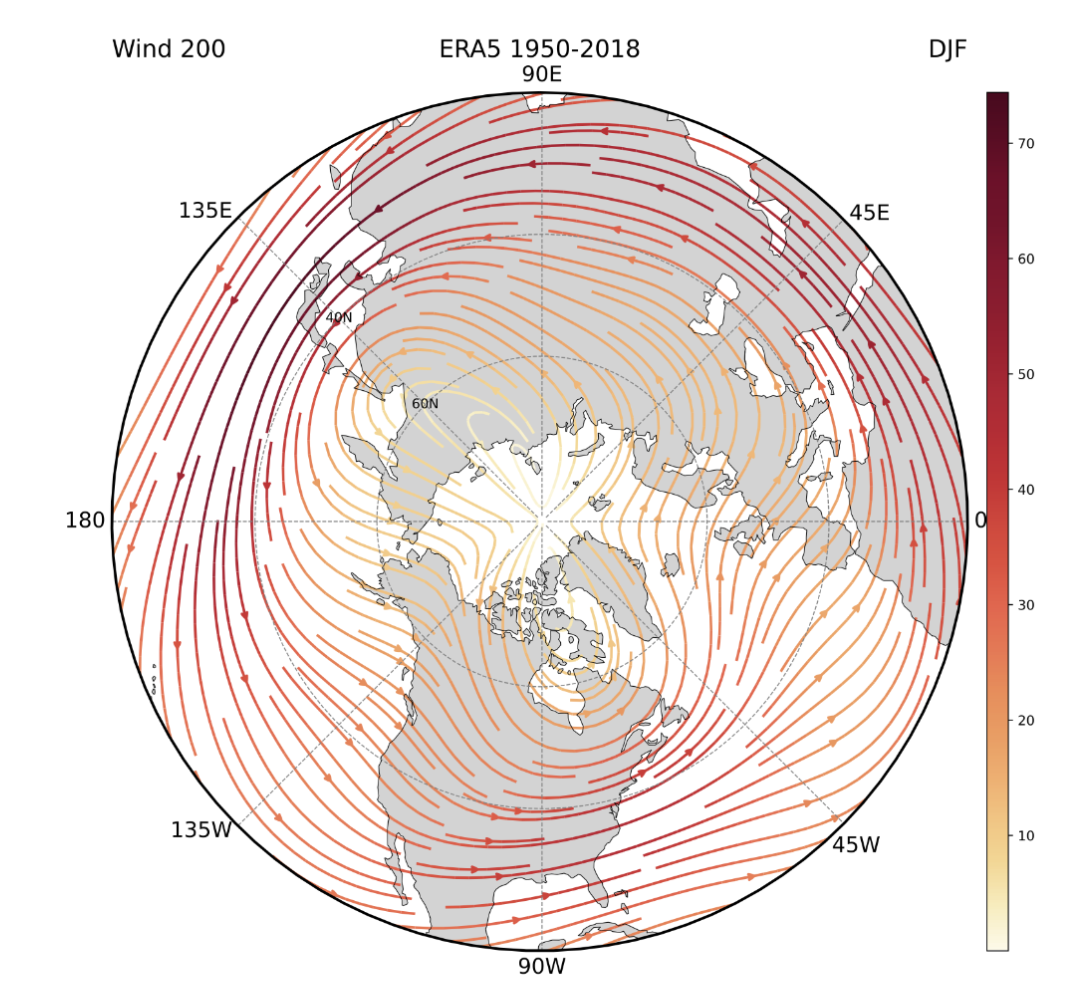
\includegraphics[width=0.5\linewidth]{uploads/Screenshot 2024-11-18 114256.png}
    \caption{ERA5-wind 200}
    \label{fig:ERA5-wind200}
\end{figure}


\subsection{Coordinate systems}\label{coordinate-systems}

\subsubsection{Spherical Coordinates}\label{spherical-coordinates}

The most commonly used coordinate system for the analysis of the
atmosphere and the oceans is a spherical coordinate system attached to
the rotating Earth (Fig. \texttt{fig:0} ). The spherical coordinates are
slightly different from the usual mathematical ones as the latitude is
measured from the equator and therefore it can take negative values. The
longitude is running west to east.

The longitude is also known as the ``zonal'' direction whereas the
latitude is also known as the "meridional" direction. Winds are
identified by the direction they are coming from, so a "westerly" wind
is coming \emph{from} the West and an "easterly" wind is coming from the
East.

This coordinate system is rotating with the Earth and therefore it
generates force terms in any dynamical equation expressed in this system
of coordinate, the Coriolis terms.

\begin{figure}[h!]
    \centering
    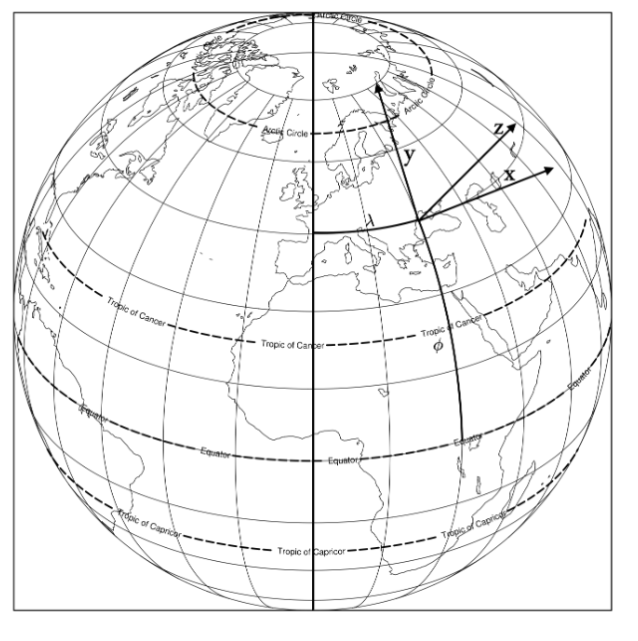
\includegraphics[width=0.5\linewidth]{uploads/Screenshot 2024-11-18 114156.png}
    \caption{Coordinate system}
    \label{fig:coordinate system3d}
\end{figure}

\subsubsection{The Beta-plane}\label{the-beta-plane}

It is sometimes convenient to shift coordinate system if the latitudinal
extension of the motion is not too great with respect to the motion
parameters as they are expressed in the adimensional numbers. When this
is possible, a tangent coordinate system is applied at a specific
latitude \(\phi_0\) and the resultant Cartesian coordinates system is
called the \(\beta\)-plane. Usually symbols \((x,y)\) are used in this
case for the zonal and meridional coordinate. In the \(\beta\)-plane the
planetary vorticity \(f\) is linearized as \(f=f_0 + \beta y\), where
\(\beta = \frac{\partial f}{\partial y}({\phi_0})\).

\subsection{Advective derivative}\label{Sec:Adv}

To describe the governing equation of the atmosphere and eventually of
the ocean we have to understand how we write the rate of change with
time of this fluid. This problem was solved by considering the fact that
the rate of change in the fluid cannot be seen as arate of change with
respect to a fixed system of coordinate because the system is moving
with the fluid itself. Therefore, first we have to find a way to
describe the change taking into account the moving system of
restaurants. These can be done by using a concept developed in the 19th
century by Euler that is called "advective derivative" that can be
obtained from a total derivative of the property,

\[\frac{d \phi}{dt} = \frac{\partial \phi}{\partial t} + \frac{\partial x}{\partial t}\frac{\partial \phi}{\partial x} + \frac{\partial y}{\partial t}\frac{\partial \phi}{\partial y}+\frac{\partial z}{\partial t}\frac{\partial \phi}{\partial z} = \frac{\partial \phi}{\partial t} + \mathbf{v}\cdot\nabla\phi\]

and so it can be defined as

\[\frac{D \varphi}{Dt} =\frac{\partial \varphi}{\partial t} + \mathbf{v}\cdot\nabla\varphi\]

in this way the moving fluid can be described by derivatives with
respect the "fixed" coordinate system, i.e. the Eulerian description.
The alternative description of the observer moving with fluid is known
as the "Lagrangian" description.



\section{Equation of motion} %this section comes from lecture6 
The motion of a physical system is governed by conservation laws: conservation of momentum, mass and energy. The conservation of momentum equation will identify the forces acting on the system. The conservation of energy will identify the processes capable of changing the energy of the system, i.e. thermodynamical processes.
The equation governing the motion of the atmosphere can be written as:

\[\begin{aligned}
&\frac{D u}{Dt} -\frac{uv \tan{\phi}}{r} +  \frac{uw}{r} = -\frac{1}{\rho r \cos{\phi}}\frac{\partial p}{\partial \lambda} + fv - \hat{f}w + F_\lambda\\
&\frac{D v}{Dt} -\frac{u^2 \tan{\phi}}{r} +  \frac{vw}{r} = -\frac{1}{\rho r }\frac{\partial p}{\partial \phi} - fu  + F_\phi\\
&\frac{D w}{Dt} -\frac{u^2+v^2}{r} = -\frac{1}{\rho }\frac{\partial p}{\partial z} -g +\hat{f}u + F_z\\
\end{aligned}\]

the \(f=2\Omega \sin{\phi}\) and \(\hat{f} = 2\Omega\cos{\phi}\) terms arise from the rotating spherical coordinate system that we have chosen, other terms are generated by the spherical geometry. Some of them are small and traditionally they can be neglected, so that we arrive at the system

\[\begin{aligned}
&\frac{D u}{Dt} - v\left(f +  \frac{u \tan{\phi}}{a}\right)  = -\frac{1}{\rho a \cos{\phi}}\frac{\partial p}{\partial \lambda}   + F_\lambda\\
&\frac{D v}{Dt} + u\left( f + \frac{u \tan{\phi}}{a}\right)  = -\frac{1}{\rho a}\frac{\partial p}{\partial \phi}  + F_\phi\\
&\frac{D w}{Dt}  = -\frac{1}{\rho }\frac{\partial p}{\partial z} -g  + F_z\\
\end{aligned}\]

where we have also used the \emph{Shallowness Approximation} by assuming \(r = a +z \approx a\), where \(a\) is the Earth radius.

However the advective derivative must be expressed in spherical cordinates

\[\frac{D }{Dt} = \frac{\partial }{\partial t} + \frac{u}{a\cos{\phi}}\frac{\partial }{\partial \lambda} +\frac{v}{a}\frac{\partial }{\partial \phi} + w\frac{\partial }{\partial z}\]

so that the velocity components are

\[\begin{aligned}
&u = a\cos{\phi\frac{\partial \lambda}{\partial t}}\\
&v = a \frac{\partial \phi}{\partial t}\\
&w = \frac{\partial z}{\partial t}
\end{aligned}\]

These equation govern the mechanical behaviour of the atmosphere, and we will see in a different form, also of the ocean. There three forces in action: pressure gradient, rotation via the Coriolis force and gravity.

The equation are not complete,we have three equation but five variables, so we need to find the missing relations. We are using the basic conservation principles, the latter equations describe the conservation
of momentum, we can exploit the conservation of mass. The mass of the fluid must be conserved locally, because there are now sinks or sources in the atmosphere itself, so we want to write the mass of a volume of
atmosphere fixed in space as

\[M = \int_V  \rho \,dV\]

the mass in the volume can only change if there is a flux of mass at surface \(S\),

\[\frac{\partial }{\partial t} \int_V  \rho \,dV = -\int_S \rho\mathbf{v}\cdot n \, dS\]

using the divergence theorem however we have

\[\frac{\partial }{\partial t} \int_V  \rho \,dV = -\int_V \nabla\cdot(\rho\mathbf{v}) \,dV\]

because the volume is not changing with time we can bring the derivative inside the integral and we get

\[\int_V  \frac{\partial \rho}{\partial t}+\nabla\cdot(\rho\mathbf{v}) \,dV = 0\]

but the volume is arbitrary, so it must be that

\[\frac{\partial \rho}{\partial t}+\nabla\cdot(\rho\mathbf{v}) = 0\]

is valid locally.

We have still at our disposal the conservation of thermodynamical energy and so we can also use

\[C_v\frac{D T}{Dt} = -p\frac{D }{Dt}\left(\frac{1}{\rho}\right)+ Q\]

where we included the temperature and heating/cooling term \(Q\). The state variable are then linked by the state equation

\[p = \rho R T\]

where \(R\) is the gas constant for dry air.

We can use the equation of state to write the energy equation ( or the temperature equation) in a different form,

\[c_v\frac{D T}{Dt} = -p\frac{D }{Dt}\left(\frac{R T}{p}\right)+ Q = -R\frac{D T}{Dt} + \frac{RT}{p}\frac{D p}{Dt} + Q\]

yielding the alternative forms ( since \(c_p = c_v +R\)),

\[c_p\frac{D T}{Dt}  - \frac{1}{\rho}\frac{D p}{Dt} = Q\]

For adiabatic processes \(Q=0\) and so

\[\begin{aligned}
&c_p\frac{D T}{Dt}  - \frac{1}{\rho}\frac{D p}{Dt} = 0\\
&\frac{c_p}{T}\frac{D T}{Dt} -\frac{R}{p}\frac{D p}{Dt} = 0\\
&\frac{D }{Dt}\log{T} - \frac{R}{c_p}\frac{D }{Dt}\log{p} = 0
\end{aligned}\]

integrating it we get

\[\log{T/T_0} - \log{\left(\frac{p}{p_0}\right)^{R/c_p}} = \text{const}\]

or

\[\frac{T}{T_0}\left(\frac{p_0}{p}\right)^{R/c_p} = \text{const}\]

so the quantity, known as \emph{potential temperature}

\[\theta = T\left(\frac{p_0}{p}\right)^{R/c_p}\]

is conserved in adiabatic processes and the thermodynamics equation can be written as

\[\frac{D \theta}{Dt} = Q\]

\paragraph{Hydrostatic balance.}
Under the action of gravity the vertical component of the pressure
gradient force balances the action of gravity, resulting in very small
vertical acceleration

\[\frac{\partial p}{\partial z} =  -g \rho\]

then if we take the vertical derivative of the eq. \texttt{Eq:logT}

\[\frac{1}{T_0}\frac{d T}{dz}\left(\frac{p_0}{p}\right)^{R/c_p} -\frac{p_0}{p^2}\frac{R}{c_p}\frac{T}{T_0}\left(\frac{p_0}{p}\right)^{R/c_p-1}\frac{d p}{dz} = 0\]

simplifying

\[\frac{d T}{dz} -\frac{p_0}{p^2}\frac{R}{c_p}T\left(\frac{p_0}{p}\right)^{-1}\frac{d p}{dz} = 0\]

or

\[\frac{d T}{dz} -\frac{1}{p}\frac{R}{c_p}T\frac{d p}{dz} = \frac{d T}{dz} +g\rho\frac{1}{p}\frac{R}{c_p}T = 0\]

but using the equation of state

\[\frac{d T}{dz} = -\frac{g}{c_p}\]

that gives how the temperature change with height under adiabatic
conditions and when the hydrostatic balance is valid. This is known as
the \emph{adiabatic lapse rate}.
\paragraph{Geostrophic balance.} Geostrophic balance is the balance between Coriolis Force and the horizontal component of the pressure gradient force.
\begin{figure}
    \centering
    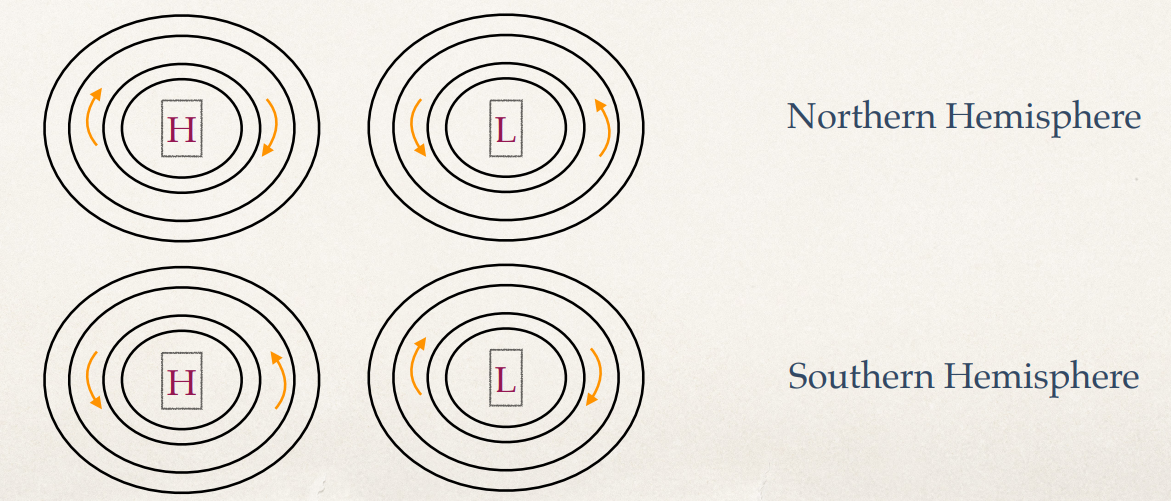
\includegraphics[width=0.5\linewidth]{uploads/Screenshot 2024-11-20 195919.png}
    \caption{Geostrophic balance}
    \label{fig:enter-label}
\end{figure}
The pressure gradient force (PGF) pushes air or water from high pressure to low pressure. The Coriolis force deflects the motion to the right in the Northern Hemisphere and to the left in the Southern Hemisphere. In geostrophic balance, these forces are equal in magnitude and opposite in direction. The geostrophic balance assumes the flow is steady and does not accelerate, so it neglects the effects of inertia. This balance is most accurate for large-scale motions (e.g., planetary or synoptic scales) where friction and other forces are negligible. Vertical motions are typically much smaller than horizontal motions and are neglected in geostrophic balance.

In geostrophic balance:
\begin{itemize}
    \item Air or water flows parallel to the isobars (lines of constant pressure) or contours of constant geopotential height. 
    \item The speed of the geostrophic flow increases with stronger pressure gradients (closer isobars).
\end{itemize}
However, on small scales (e.g., tornadoes, boundary layers), friction and other forces become important, so geostrophic balance is less accurate. Near the Equator, The Coriolis parameter ($f$) approaches zero, making the geostrophic balance invalid.



\subsection{Summary of fundamental
equations}\label{summary-of-fundamental-equations}

Summarizing our discussion, the fundamental equation that describe the
motion of the atmosphere are considered in the following approximations:
\begin{itemize}
    \item Hydrostatic approximation
    \item Shallow fluid approximation. The vertical coordinate $r$ is sustituted by $a+z(a>>z)$ except in differentiation
    \item Neglecting metric terms involving vertical velocity $w$
\end{itemize}
The first approximation is independent, the second and the third must be applied together. These primitive (non hydrostatic) equations are:
\[\begin{aligned}
&\frac{D u}{Dt} - v\left(f +  \frac{u \tan{\phi}}{a}\right)  = -\frac{1}{ a \cos{\phi}}\frac{1}{\rho}\frac{\partial p}{\partial \lambda}   + F_\lambda \\
&\frac{D v}{Dt} + u\left( f + \frac{u \tan{\phi}}{a}\right)  = -\frac{1}{a}\frac{1}{\rho}\frac{\partial p}{\partial \phi}  + F_\phi \\
&\frac{D w}{Dt}  = -\frac{1}{\rho }\frac{\partial p}{\partial z} -g  + F_z \label{Eq:PrimEq}\\
&\frac{D \theta}{Dt} = Q \\
&\frac{\partial \rho}{\partial t}+\frac{1}{a\cos{\phi}}\left[ \frac{\partial }{\partial \lambda}(\rho u) + \frac{\partial }{\partial \phi}(rv\cos{\phi} )\right] +\frac{\partial }{\partial z}(\rho w) = 0 \\
&p = \rho R T
\end{aligned}\]

where we have used the divergence in spherical coordinates.

These equations are still not closed because we will need to express the heating/cooling term \(Q\) and the friction terms \(F\) as a function of the state variables. This will require a theory of the processes that
drive them. Where \(R=287.052874 J \quad kg^{-1} K^{-1}\) is the gas constant for dry air and \(c_p = 1.005\) is the specific heat at constant pressure, \(c_v = 0.718\) is the specific heat at constant volume, \(\kappa = \frac{R}{c_p}\) and \(\gamma=c_p/c_v\) is their ratio.

For theoretical and idealized studies the set of equation projected on the \(\beta\)-plane is also used. The $\beta$-plane approximation is a simplified model used in geophysical fluid dynamics to account the variation of the Coriolis parameter $f$ with latitude, in this approximation $f$ is linearized around a reference latitude such that $f\approx f_0+\beta y$ with $y=a(\phi-\phi_0)$ is the northward displacement from the reference latitude. With the $\beta$-plane approximation, no rotation, no sphericity, neglecting the meridional coordinates, the equations become:

\[\begin{aligned}
&\frac{D u}{Dt} - fv  = -\frac{1}{\rho}\frac{\partial p}{\partial x}   + F_x \\
&\frac{D v}{Dt} + fu = -\frac{1}{\rho}\frac{\partial p}{\partial y}  + F_y \\
&\frac{D w}{Dt}  = -\frac{1}{\rho }\frac{\partial p}{\partial z} -g  + F_z \\
&\frac{D \theta}{Dt} = Q\\
&\frac{\partial \rho}{\partial t}+\nabla\cdot(\rho\mathbf{v}) = 0\\
&p = \rho R T
\end{aligned}\]

and the gradient operator is the cartesian operator

\[\nabla = \frac{\partial }{\partial x} + \frac{\partial }{\partial y} + \frac{\partial }{\partial z}\]

and the advective derivative is then

\[\frac{D }{Dt} = \frac{\partial }{\partial t} + u\frac{\partial }{\partial x} + v\frac{\partial }{\partial y} + w\frac{\partial }{\partial z}\]

The first set of fundamental equations that we encounter is the conservation of Momentum (\textbf{Navier.Stokes equations)}. The Navier-Stokes equations describe the motion of fluid substances like air and water. They account for forces due to pressure, viscosity, and external forces such as gravity. This set of equations is key to understanding how winds, ocean currents, and other flows evolve due to internal and external forces. In a rotating frame of reference, specifically describing the motion of a fluid (e.g. the atmosphere or ocean currents) the principal equation can be declined in the different directions: longitude, latitude and vertical directions. 

The left-hand side of the equations begins with material derivative of the velocity components ($u$ in the east-west direction, associated with longitude; $v$ north-south velocity component, associated with latitude, $w$ is the vertical velocity component).
The material derivative includes both the local rate of change and the advection (transport) of the velocity. This term tells us how the velocity of a fluid parcel changes over time, taking into account both temporal changes and the movement of the parcel.

The second term on the left represents the COriolis force and the centrifugal force in the rotating reference frame of the Earth. $f$ is the Coriolis parameter, which depends on the latitude $\phi$ and is given by $f=2\Omega\sin\phi$ where $\Omega$ is the angular velocity of the Earth and $\phi$ is the latitude. The Coriolis force is proportional to the velocity and acts perpendicular to the motion of the fluid, deflecting the fluid in different directions depending on the hemisphere.

On the right side of the equations we find the pressure gradient force in the longitudinal (first) and latitudinal (second) directions, which drives fluid motion due to differences in pressure. The terms $F_{\lambda}$, $F_{\phi}$ and $F_{z}$ represent an additional force term that could represent any other forces acting on the fluid parcel in the longitudinal, latitudinal and vertical direction. It might include friction, external forces, or any other model-specific forces not accounted for in the other terms.
\begin{equation}
    \frac{Du}{Dt}-v\left(f+\frac{u\tan\phi}{a}\right)=-\frac{1}{a\cos\phi}\frac{1}{\rho}\frac{\partial p}{\partial\lambda}+F_{\lambda}
\end{equation}
The term $\frac{u\tan\phi}{a}$ accounts for the centrifugal force resulting from the Earth's rotation. Here, $u$ is the east-west velocity, $\phi$ is the latitude, and $a$ is the Earth's radius. The centrifugal force is stronger near the equator, and this term adjusts the Coriolis effect to account for that.
$\frac{\partial p}{\partial\lambda}$ is the derivative of pressure with respect to longitude ($\lambda$), indicating how pressure changes as you move east or west. The term $a\cos\phi$ accounts for the spherical geometry of the Earth and the fact that distances between lines of longitude vary with latitude (they are widest at the equator and shrink towards the poles). This term describes the acceleration due to the horizontal pressure gradient in the longitudinal direction, with the pressure gradient force causing flow from regions of higher to lower pressure.
\begin{equation}
    \frac{Dv}{Dt}+u\left(f+\frac{v\tan\phi}{a}\right)=-\frac{1}{a}\frac{1}{\rho}\frac{\partial p}{\partial\phi}+F_{\phi}
\end{equation}
The term $\frac{v\tan\phi}{a}$ is the centrifugal force term in the north-south direction, considering Earth's curvature. $\frac{p}{\phi}$ represents the pressure gradient in the latitude direction, and it drives motion from high to low pressure.


Note that the Coriolis term arises due to the rotation of the Earth, which introduces an apparent force in a rotating reference frame. This term depends explicitly on the latitude because of how the Earth's rotation affects the direction and magnitude of the Coriolis effect at different points on the Earth's surface. The Coriolis force explicitly depends on the sine of the latitude, as the projection of $\Omega$ onto the local horizontal plane is $\Omega\sin\phi$ (the latitude $\phi$ determines the angle between the Earth's rotational axis and the local vertical. $\Omega$ is the angular velocity vector of Earth's rotation, it points along the axis of rotation (towards the North Pole). At the Equator $\phi=0°$ the Coriolis effect is perpendicular to $\Omega$ and has a max horizontal effect. At the poles ($\phi=\pm 90°$) the effect aligns with $\Omega$, and only the vertical motion is affected.

In the vertical direction:
%check if these are correct
\begin{equation}
    \frac{Dw}{Dt}=-\frac{1}{\rho}\frac{\partial p}{\partial z}-g+F_z
\end{equation}
While the Coriolis force primarily affects horizontal motion, the vertical component of the Coriolis force is negligible because $\Omega$ is nearly parallel to the vertical axis in most regions. In rotating systems like the atmosphere or oceans, vertical Coriolis terms are often ignored. $g$ acts downward and opposes upward motion. 
\\
 

The equation
\begin{equation}
    \frac{D\theta}{Dt}=Q
\end{equation}

says that the rate of change of $\theta$ (the material derivative) experienced by a fluid parcel moving through space is equal to the source term $Q$. This equation describes the rate of change of a scalar quantity (like temperature or moisture) \textbf{for a fluid parcel} moving through space. The term $Q$ could represent a source of energy or mass, such as heat from the sun or moisture added by evaporation. In the context of a weather or climate model, this would represent how temperature (or another variable) changes as the air parcel moves and as energy is gained or lost. 
This equation is a general form for describing the time evolution of a scalar quantity (like T or moisture) in a moving fluid, where the change in that quantity is driven by external sources or sinks.
\\



The conservation of mass or continuity equation ensures that the mass is conserved in the system. For the atmosphere or the ocean, it wxpresses how the density of air or water changes over time due to processes like flow and diffusion.
\begin{equation}
    \frac{\partial\rho}{\partial t}+\nabla\cdot(\rho\vec{v})=0
\end{equation}
$\nabla\cdot(\rho\vec{v})$ represents the divergence of the mass flux, which accounts for the movement of the mass.
\\
The last one is the equation of state for atmospheric or oceanic models links pressure, density and temperature of the fluid. The ideal gas law is typically used:
\begin{equation}
    p=\rho RT
\end{equation}

\subsection{Linear solutions}
Search for solution that describe small oscillation away from a basic state, in this case assumed in hydrostatic balance: 
\begin{equation}
    \frac{\partial p_0}{\partial z}=-g\rho_0=-\frac{gp_0}{RT_0}
\end{equation}
With the further assumption of isotherm atmosphere we can integrate to get: 
\begin{equation}
    p_0(z)=p_Re^{-z/H}
\end{equation}
and $H=\frac{RT_0}{g}$ is the scale height. \\


The primitive equations are a system of nonlinear partial differential equations governing fluid motion on a rotating sphere. These include momentum equations, continuity (mass conservation), thermodynamic equations and the equation of state. Since solving the full nonlinear system is often impractical, the system is linearized to analyze small deviations (or perturations) from a reference state (steady flow or a state of rest). Assume the flow can be separated into a basic state and a perturbation:
\begin{align*}
    u=u_0+u'\\
    v=v_0+v'\\
    \theta=\theta_0+\theta'\\
    p=p_0+p'
\end{align*}
The resulting linearized primitive equations describe how perturbations evolve over time and space (linear equations are obtained for the prime variables neglecting all terms quadratic in perturbation). 
For instance, the pressure gradient becomes:
\begin{equation}
    \frac{1}{\rho_0+\rho'}\nabla(p_0+p')+g\hat{k}\approx\frac{1}{\rho_0+\rho'}\nabla p'+g\hat{k}=\frac{1}{\rho_0}\frac{1}{1+\frac{\rho'}{\rho_0}}\nabla p'+g\hat{k}=\frac{1}{\rho_0}\nabla p'+g\hat{k}
\end{equation}
and the potential temperature:
$$
    \theta=T\left(\frac{p_R}{p}\right)^k=\frac{p_R^k}{R}\frac{p^{1-k}}{\rho}\approx\theta_0\left[1+\frac{1}{\gamma}\left(\frac{p'}{p_0}\right)-\frac{\rho'}{\rho_0}\right]
$$
hence, 
\begin{equation}
    \frac{\theta'}{\theta_0}=\frac{1}{\gamma}\frac{p'}{p_0}-\frac{\rho'}{\rho_0}
\end{equation}
with $\gamma=\frac{c_p}{c_v}$, $k=\frac{R}{c_v}$, $R=c_p-c_v$.

The linearized system often supports wave-like solutions. These solutions arise naturally due to the restoring forces in the equations, such as: 
\begin{itemize}
    \item Pressure gradient drives the oscillations through compressibility or bouyancy 
    \item Coriolis force introduces rotational effects leading to inertial and planetary waves
    \item Gravity acts as a restoring force for vertical displacement, driving internal gravity waves.
\end{itemize}

We take the equations for perturbation: 
\begin{align*}
    \frac{\partial u}{\partial t}+U\frac{\partial u}{\partial x}+\frac{1}{\rho_0}\frac{\partial p}{\partial x}=0\\
     \frac{\partial w}{\partial t}+U\frac{\partial w}{\partial x}+\frac{1}{\rho_0}\frac{\partial p}{\partial z}+g\frac{\rho}{\rho_0}=0\\
     \frac{\partial\rho}{\partial t}+U\frac{\partial\rho}{\partial x}+w\frac{\partial\rho_0}{\partial z}+\rho_0(\frac{\partial u}{\partial x}+\frac{\partial w}{\partial z})=0\\
     \frac{\partial\theta}{\partial t}+U\frac{\partial\theta}{\partial x}+w\frac{\partial\theta_0}{\partial z}=0\\
     \frac{\theta}{\theta_0}+\frac{\rho}{\rho_0}+\frac{1}{\gamma}\frac{p}{p_0}=0
\end{align*}

%slides 24-29 LEC6 non le ha molto cagate
Basically to find solutions, assume the perturbations take the form of plane waves:
$$\mathbf{u'}(x,t)=\hat{\mathbf{u}}e^{i(\mathbf{k}\cdot\mathbf{x}-\omega t)}$$
where $\mathbf{\hat{u}}$ is the amplitude of the perturbation, $\mathbf{k}$ is the wavevector, $\omega$ the angular velocity. Substituing this kind of wave into the linearized equations leads to a dispersion relation, which relates $\omega$ to $\mathbf{k}$ and the physical parameters of the system (Coriolis, ...).
The perturbation equations link the restoring forces to wave properties:
\begin{enumerate}
    \item The momentum equations describe how velocity perturbations interact with pressure gradients and Coriolis forces.
    \item The continuity equation ensures mass conservation, connecting velocity and density perturbations.
    \item The thermodynamic equation relates temperature, pressure and density perturbations
\end{enumerate}
Imposing the hydrostatic approximation from the beginning would mean putting to zero from the start the time derivative of $w$ in the momentum equation in the vertical. This basically is equivalent to say that we are removing the explicit dependence of the vertical velocity on time and therefore the 


\paragraph{Advective derivative in rotating coordinates}


\paragraph{Vertical coordinates}
The original vertical coordinate was the Z coordinate that is simply the
geometric height. However because of the hydrostatic balance it was thought
convenient to use the pressure as a vertical coordinate. This choice as the
problem that the surface pressure intersects the surface especially over
mountains creating problems numerically in the definition of the boundary
condition.
Phillips (1957) proposed to use a normalised pressure coordinate, $\sigma=\frac{p}{p_s}$
\begin{figure}[h!]
    \centering
    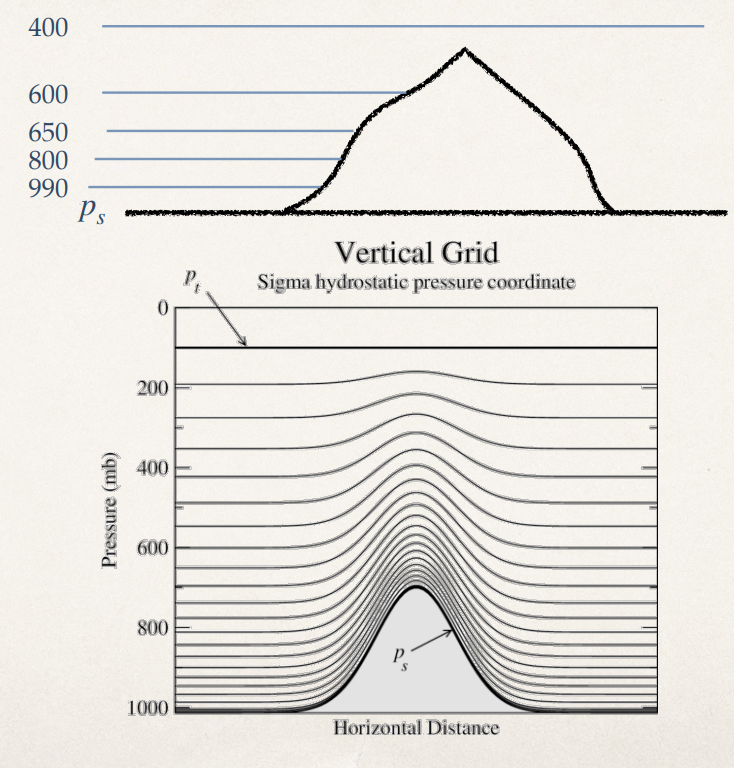
\includegraphics[width=0.5\linewidth]{uploads/Screenshot 2024-11-19 143432.png}
    \caption{Pressure coordinates vs sigma coordinates: $\sigma=\frac{p-p_T}{p_s-p_T}$}
    \label{fig:enter-label}
\end{figure}
\paragraph{Hybrid coordinates}
It is a sigma coordinates close to the ground, but smoothly transform into a
pressure coordinate far from the ground

\paragraph{Vertical Advection}%check
\begin{equation}\label{eq.vertical advection}
    \left(\sigma\frac{\partial U}{\partial\sigma}\right)=\alpha_k
\end{equation}

